\section{Contenedor para actividades de ciencia de datos basado en Python}

\subsection{Descripción}

Contenedor partiendo de una imagen base de Ubuntu al que se le añade Python con distintos paquetes de ciencia de datos, concretamente:
\begin{itemize}
    \item pandas
    \item scikit-learn
    \item seaborn
    \item scipy
    \item numpy
    \item matplotlib
    \item xlrd
\end{itemize}

\subsection{Archivo Dockerfile}

\begin{figure}[H]\center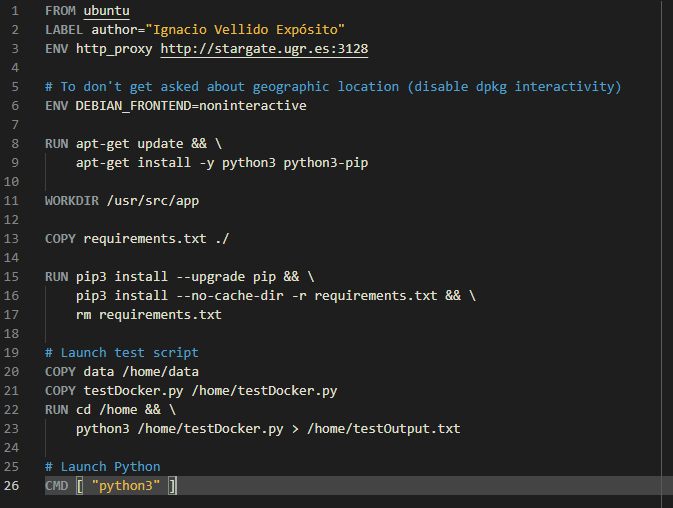
\includegraphics[width=.95\linewidth]{img/python/p0.png}\caption{}\end{figure}

\begin{figure}[H]\center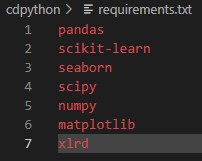
\includegraphics[width=.65\linewidth]{img/python/p0-2.png}\caption{Archivo con los paquetes a instalar}\end{figure}

Para la construcción del archivo Dockerfile se parte de las recomendaciones de \url{https://hub.docker.com/_/python} y se adapta para una instalación base de Ubuntu.

\subsection{Proceso de construcción}

\subsubsection{En hadoop.ugr.es}

\begin{figure}[H]\center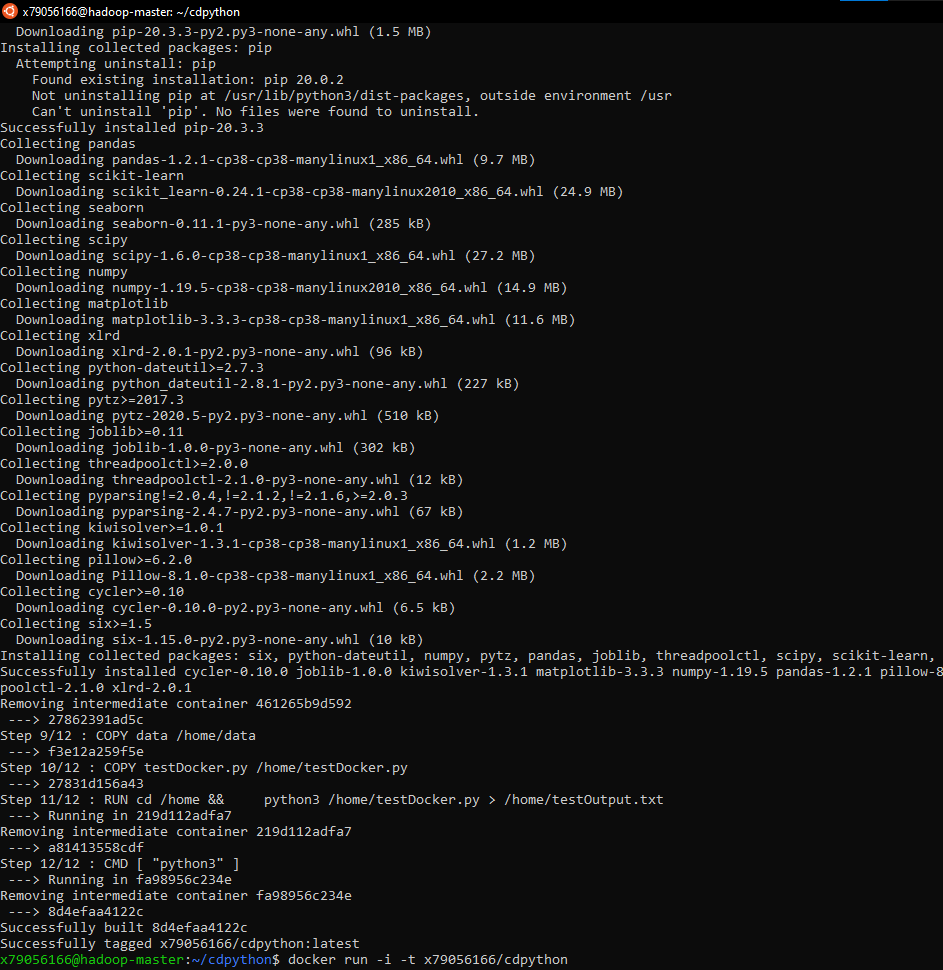
\includegraphics[width=.95\linewidth]{img/python/p1.png}\caption{Construcción de la imagen}\end{figure}

\begin{figure}[H]\center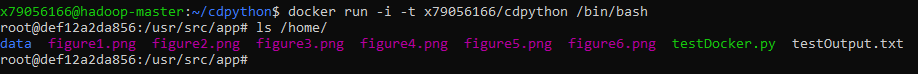
\includegraphics[width=.95\linewidth]{img/python/p2.png}\caption{Lanzando la imagen}\end{figure}

\begin{figure}[H]\center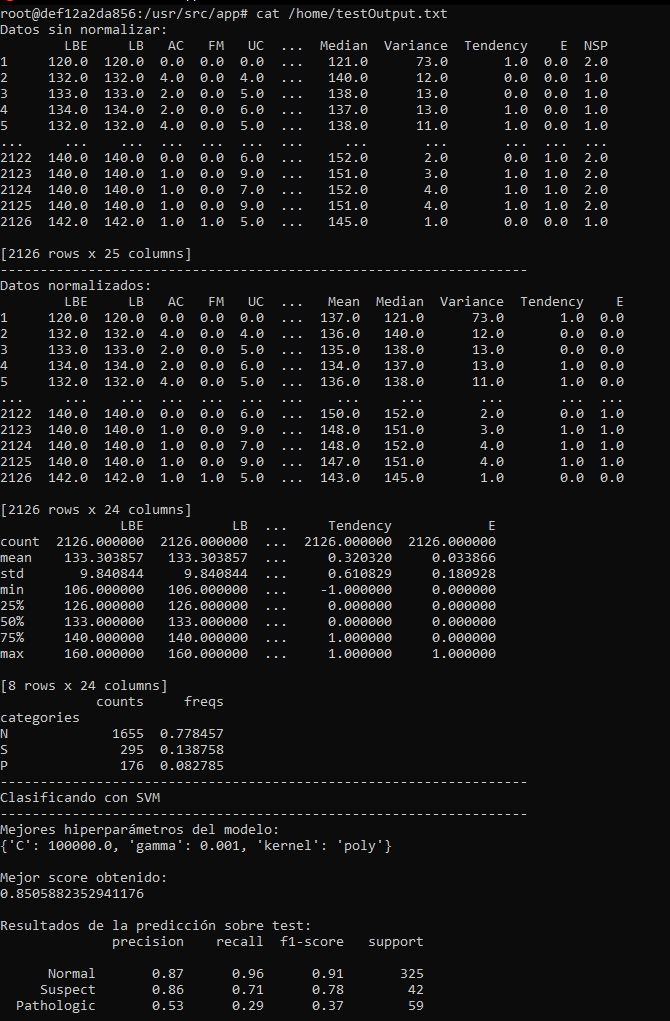
\includegraphics[width=.95\linewidth]{img/python/p3.png}\caption{Contenido de la imagen}\end{figure}

\begin{figure}[H]\center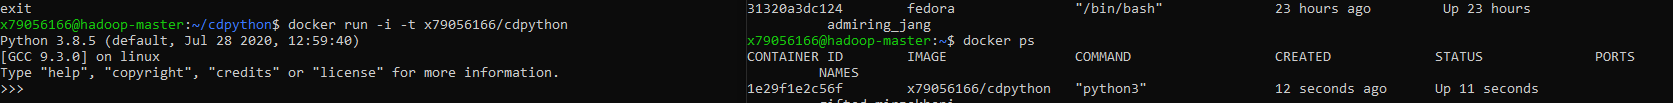
\includegraphics[width=.95\linewidth]{img/python/p5.png}\caption{Comprobando ejecución}\end{figure}

\subsubsection{En Azure}

\begin{figure}[H]\center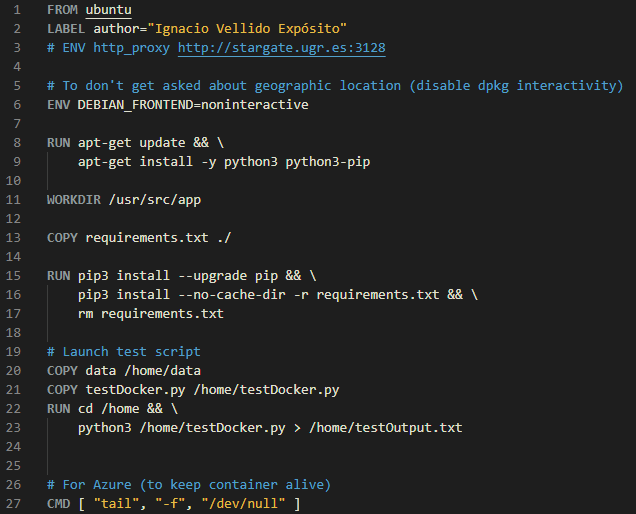
\includegraphics[width=.95\linewidth]{img/python/p10.png}\caption{Dockerfile desplegado en Azure}\end{figure}

\begin{figure}[H]\center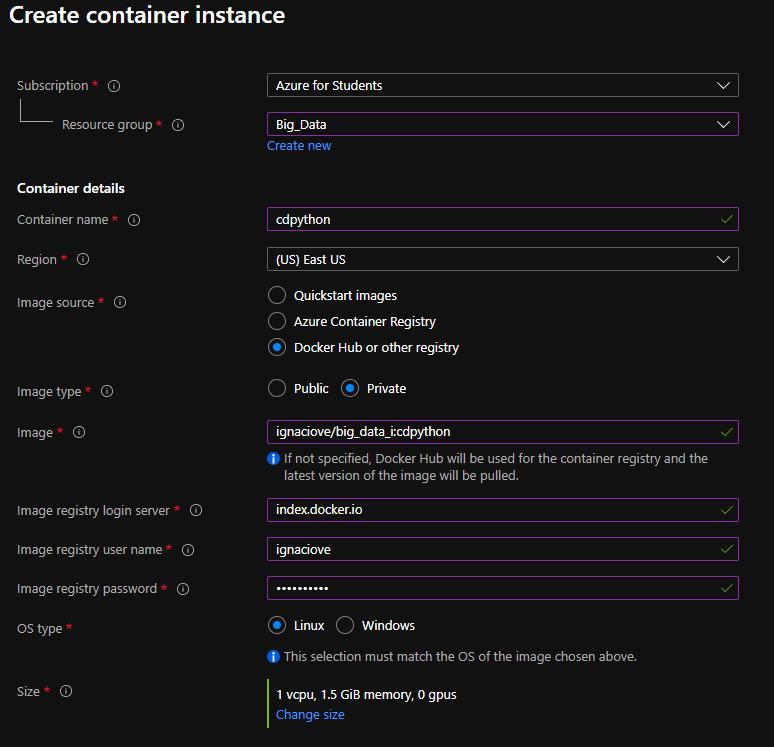
\includegraphics[width=.95\linewidth]{img/python/p7.png}\caption{Despliegue del contenedor en Azure}\end{figure}

% \begin{figure}[H]\center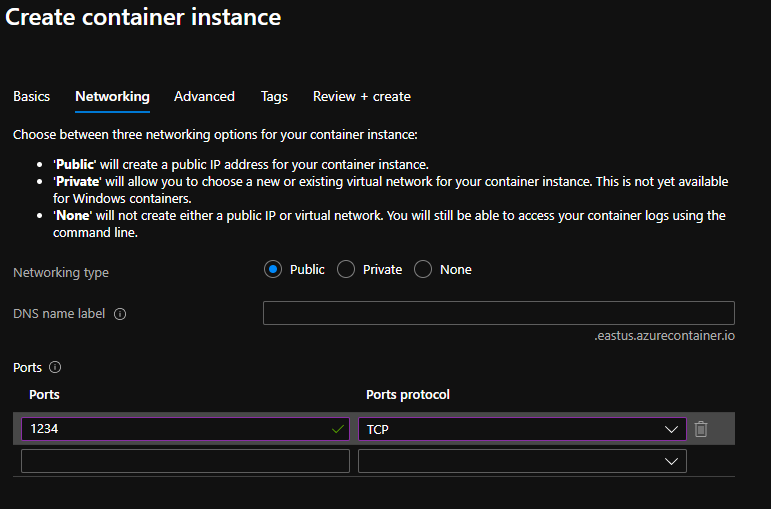
\includegraphics[width=.95\linewidth]{img/python/p8.png}\caption{Indicando puerto a abrir}\end{figure}

\begin{figure}[H]\center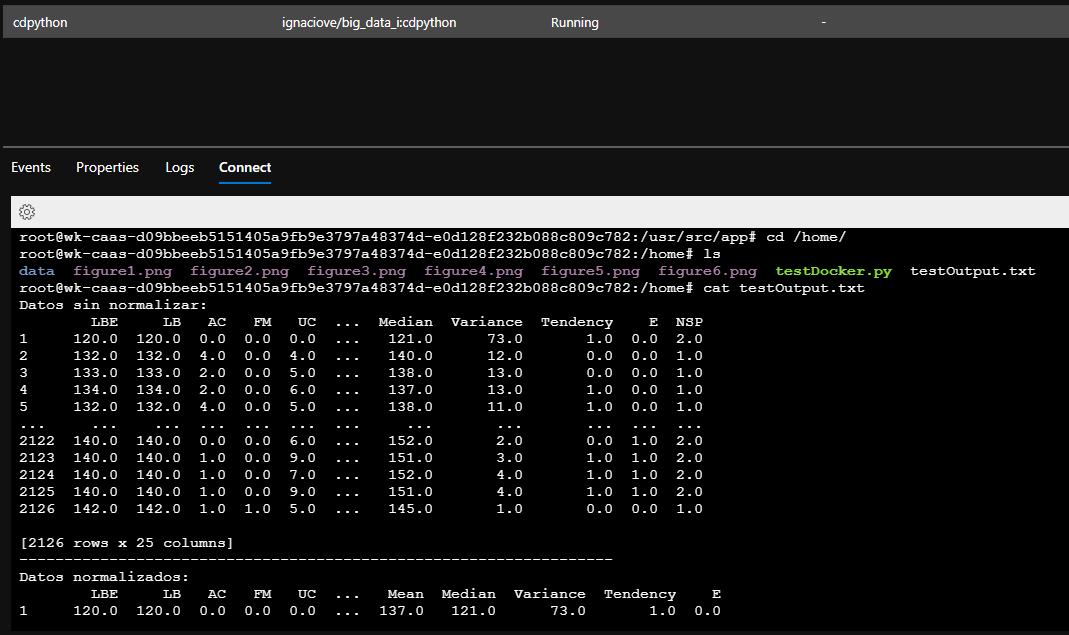
\includegraphics[width=.95\linewidth]{img/python/p9.png}\caption{Imagen del contenedor en ejecución}\end{figure}

% \begin{figure}[H]\center\includegraphics[width=.95\linewidth]{img/python/p11.png}\caption{Acceso al contendor desde SSH}\end{figure}

\subsection{Evaluación}

Para evaluar el correcto funcionamiento se lanza el siguiente script, que carga los paquetes instaladas y realiza un aprendizaje sobre un conjunto de datos con SVM.

\begin{figure}[H]\center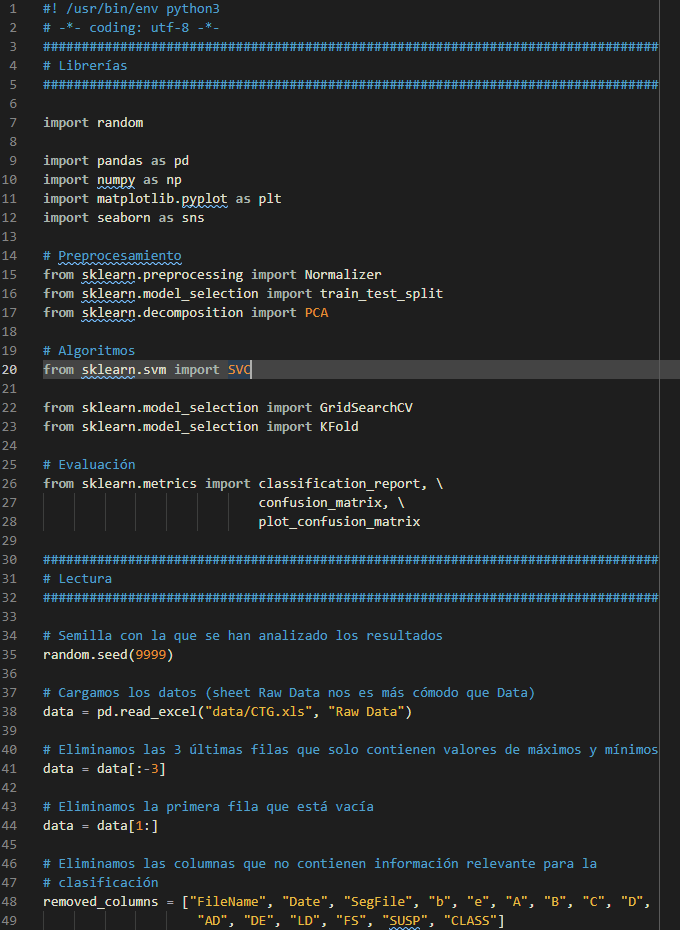
\includegraphics[width=.95\linewidth]{img/python/p6.png}\caption{Script de prueba}\end{figure}